\section{Architecture for Partial Monitoring}
\label{sec:monitoring_dift_drop.dropping}

% Example monitor
\begin{figure}
  \begin{center}
    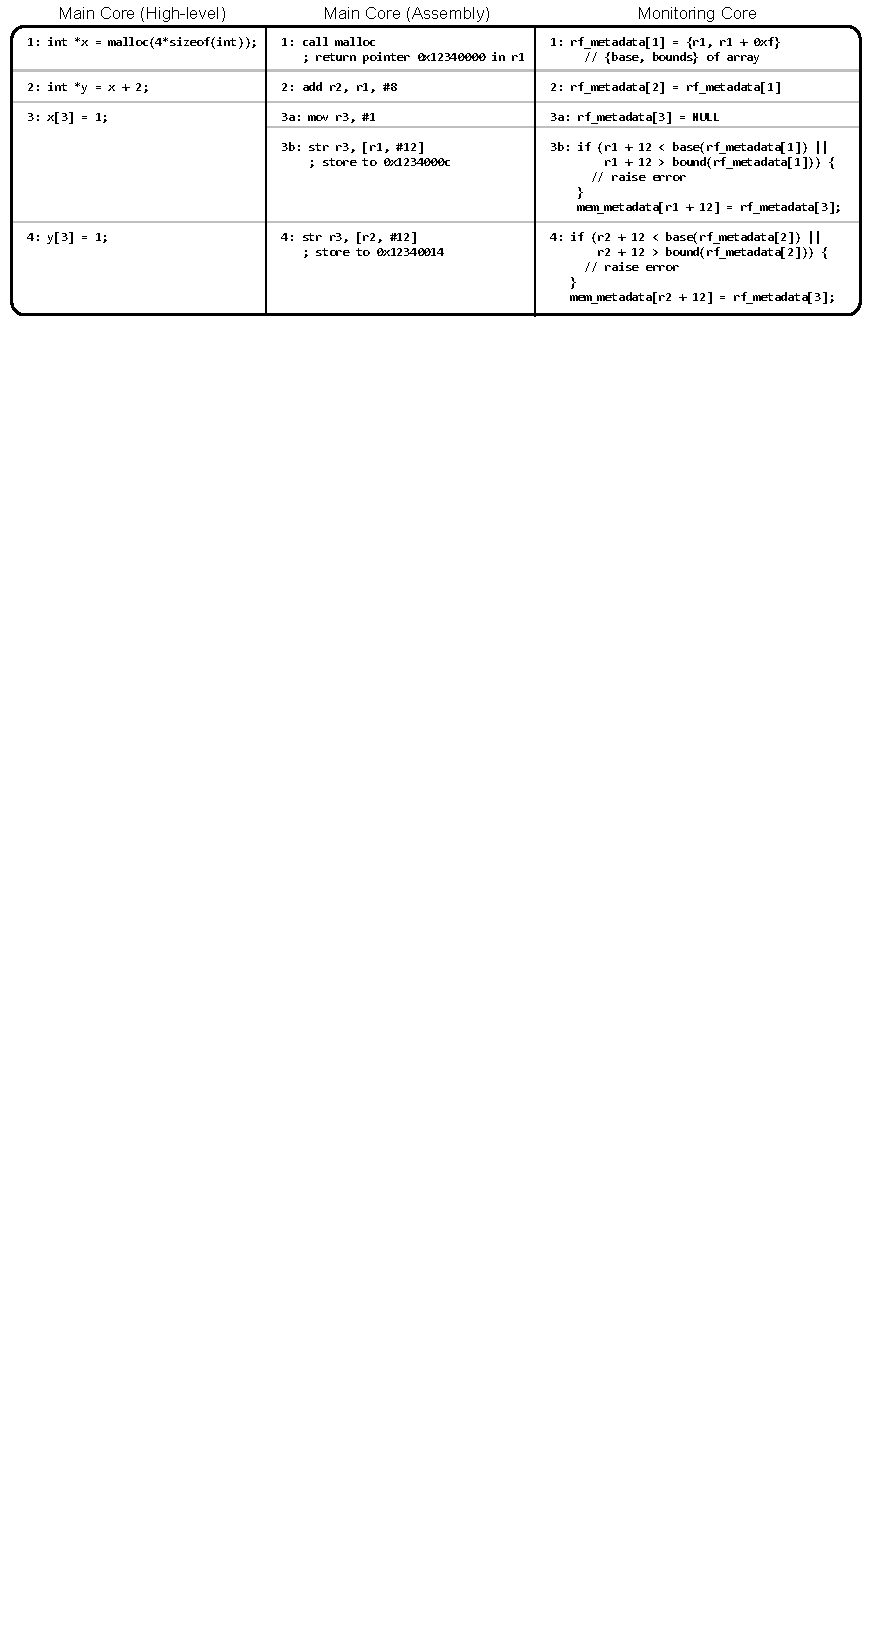
\includegraphics{figs/example_full.pdf}
    \caption{Example of array bounds check monitor.}
    \label{fig:monitoring_dift_drop.dropping.example_full}
  \end{center}
\end{figure} 

In this section, we present our hardware architecture that enables partial
monitoring for adjustable overhead. We will revisit the array bounds check
monitor and example code sequence that was shown in
Figure~\ref{fig:background.monitoring.example_full} from
Section~\ref{sec:background.monitoring.example}. This example is repeated
in Figure~\ref{fig:monitoring_dift_drop.dropping.example_full} for easy
reference.

\subsection{Effects of Dropping Monitoring}
\label{sec:monitoring_dift_drop.dropping.false_neg_pos}

Our goal is to drop some monitoring operations in order to reduce the overhead
of run-time monitoring. This dropping can affect the functionality of the
monitoring scheme. There are three possible outcomes for dropping a monitoring
operation. The first is that there is no difference in operation from the
original execution. For example, if we drop line 3b from our array bounds check
example (Figure~\ref{fig:monitoring_dift_drop.dropping.example_full}), then the
check on accessing {\tt x+12} is skipped. However, this is a valid access and
so skipping the check does not change anything.

On the other hand, if the monitoring for accessing memory location {\tt y+12}
on line 4 is skipped, then a false negative occurs. Originally, the monitor
would catch this access as an out-of-bounds access and raise an error. However,
if the monitoring operation for this is dropped, then the error is not
detected. This reflects the trade-off that we make in order to reduce overhead.
Instead of either 100\% coverage with all the associated overhead or no
coverage and no overhead, we enable middle points of partial coverage with some
fraction of the full overhead.

The final possible outcome of dropping a monitoring operation is a false
positive.  For example, suppose the monitoring for line 1 is dropped, causing
the bound information for pointer {\tt x} to never be set. The result is that
when the access using {\tt x} is checked on line 3b, an error will be raised.
This creates a false positive where an error is incorrectly raised. Although
false negatives are part of the trade-off we make to reduce overhead, we need
to prevent false positives.

\subsection{Invalidation for Preventing False Positives}
\label{sec:monitoring_dift_drop.dropping.prevent_false_pos}

% Example with invalidation
\begin{figure}
  \begin{center}
    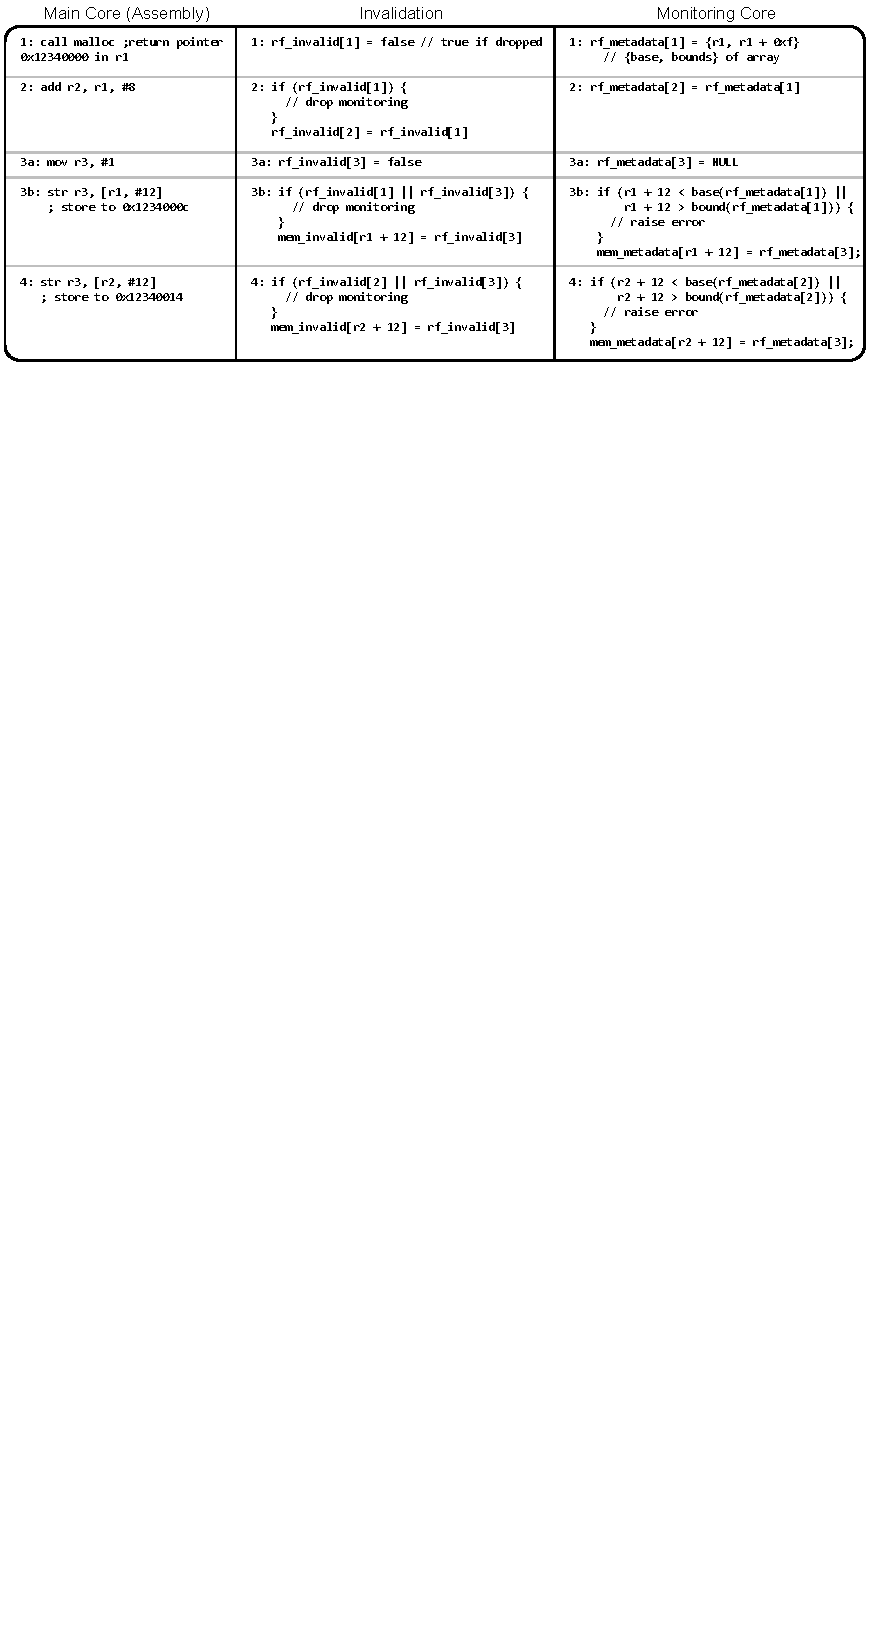
\includegraphics{monitoring_dift_drop/figs/example_invalid.pdf}
    \caption{Example of using invalidation information to prevent false positives.}
    \label{fig:monitoring_dift_drop.dropping.example_invalid}
  \end{center}
\end{figure}

The key cause of false positives is dropping monitoring operations that update
metadata. Dropping monitoring operations that check for an error (such as the
check for line 4 in
Figure~\ref{fig:monitoring_dift_drop.dropping.example_full}) can only cause
false negatives and will never cause false positives. On the other hand,
skipping monitoring operations that update metadata can lead to false positives
and false negatives.  Essentially, when an update operation is skipped, we can
no longer trust the corresponding metadata. Thus, our general approach for
preventing false positives is to associate a 1-bit invalidation flag with each
metadata in order to mark these metadata as valid or invalid, as was done for
the hard real-time monitoring architecture presented in
Chapter~\ref{chap:monitoring_hard_drop}. Furthermore, this
invalidation information is propagated in the same way that metadata is.
Figure~\ref{fig:monitoring_dift_drop.dropping.example_invalid} shows an example
of associating invalidation flags with metadata. Suppose that the monitoring
for line 1 is dropped in order to meet the overhead target. When a monitoring
event is dropped, metadata that would have been updated is marked as invalid.
In this case, instead of the normal operation of marking {\tt rf\_invalid[1]}
as {\tt false}, it is instead marked as {\tt true}. Thus, when line 3 is
reached, the monitoring event is dropped since {\tt rf\_invalid[1]} is marked
as true. Note that in this case, line 2 also propagates this invalidation flag
to {\tt rf\_invalid[2]} and causes the check performed on line 4 to also be
dropped. This is necessary because an error would have been raised even if the
access on line 4 was within bounds.

\subsection{Dataflow Engine for Preventing False Positives}
\label{sec:monitoring_dift_drop.dropping.arch}

% Dataflow engine high-level
\begin{figure}
  \begin{center}
    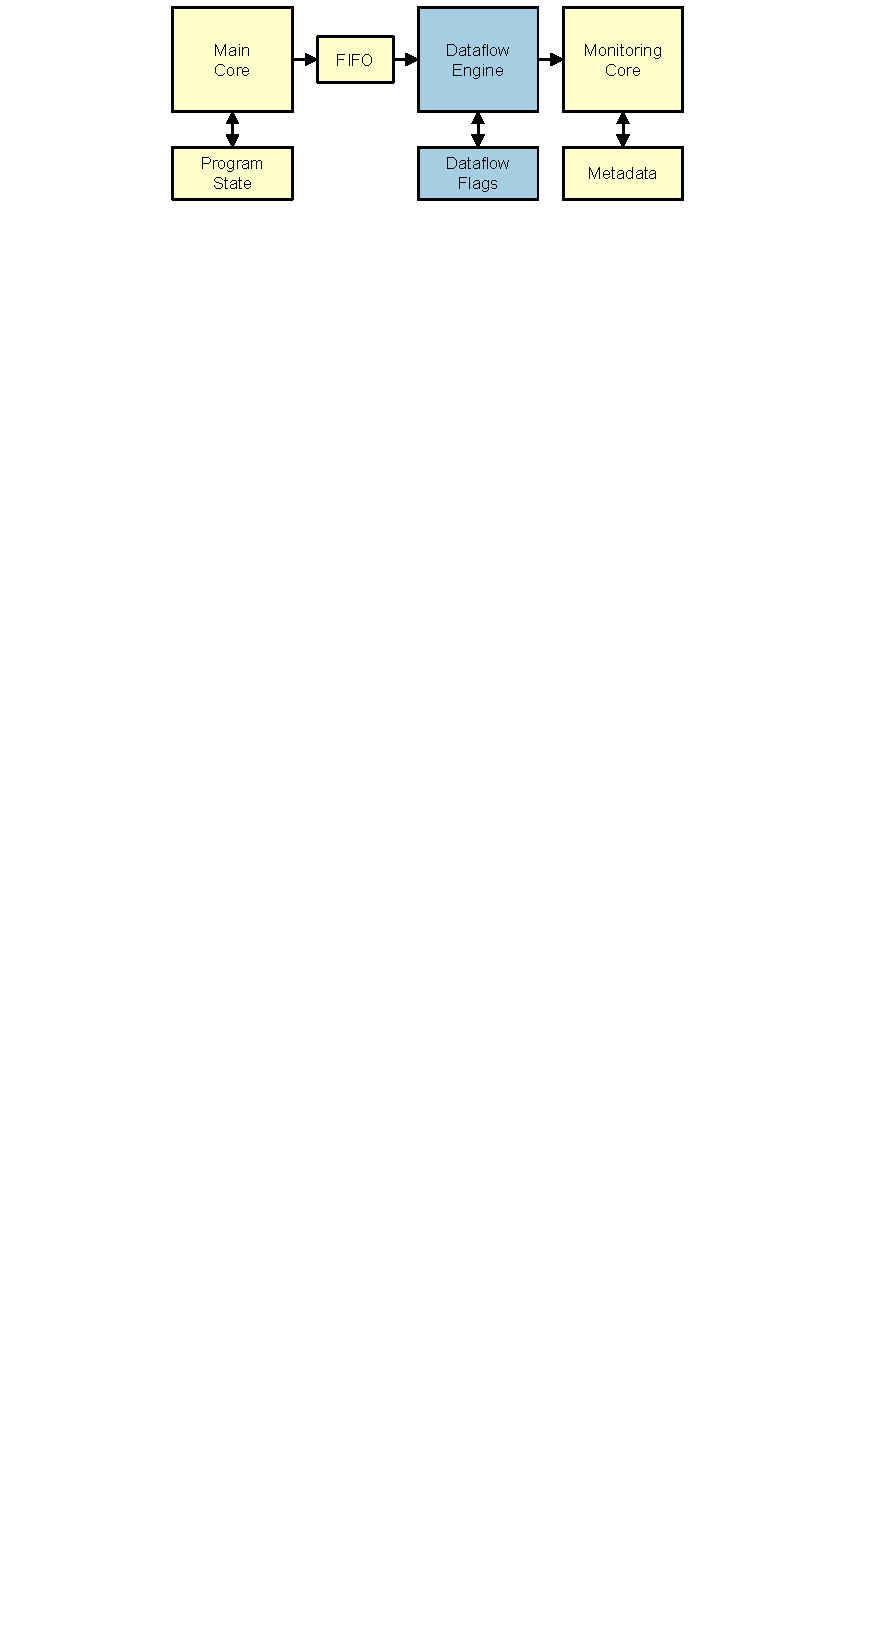
\includegraphics{monitoring_dift_drop/figs/dataflow_overview.pdf}
    \caption{Hardware support for dropping.}
    \label{fig:monitoring_dift_drop.dropping.dataflow_overview}
  \end{center}
\end{figure}

Although the functionality of dropping and invalidation could be implemented on
the monitoring core, this is unlikely to be much faster than performing the full
monitoring operations.  Instead, in order to efficiently support dropping
monitoring events and to prevent false positives, we propose to insert a
hardware module between the main core and the monitoring core (see
Figure~\ref{fig:monitoring_dift_drop.dropping.dataflow_overview}).  This module
handles the invalidation operations shown in the middle column of
Figure~\ref{fig:monitoring_dift_drop.dropping.example_invalid}.  There are two
operations that are done for handling invalidation information:

\begin{enumerate}
  \item Propagate invalidation flags, following the dataflow of metadata.
  \item Filter out monitoring operations based on invalidation flags.
\end{enumerate}

% Detailed architecture of dataflow engine
\begin{figure}
  \begin{center}
    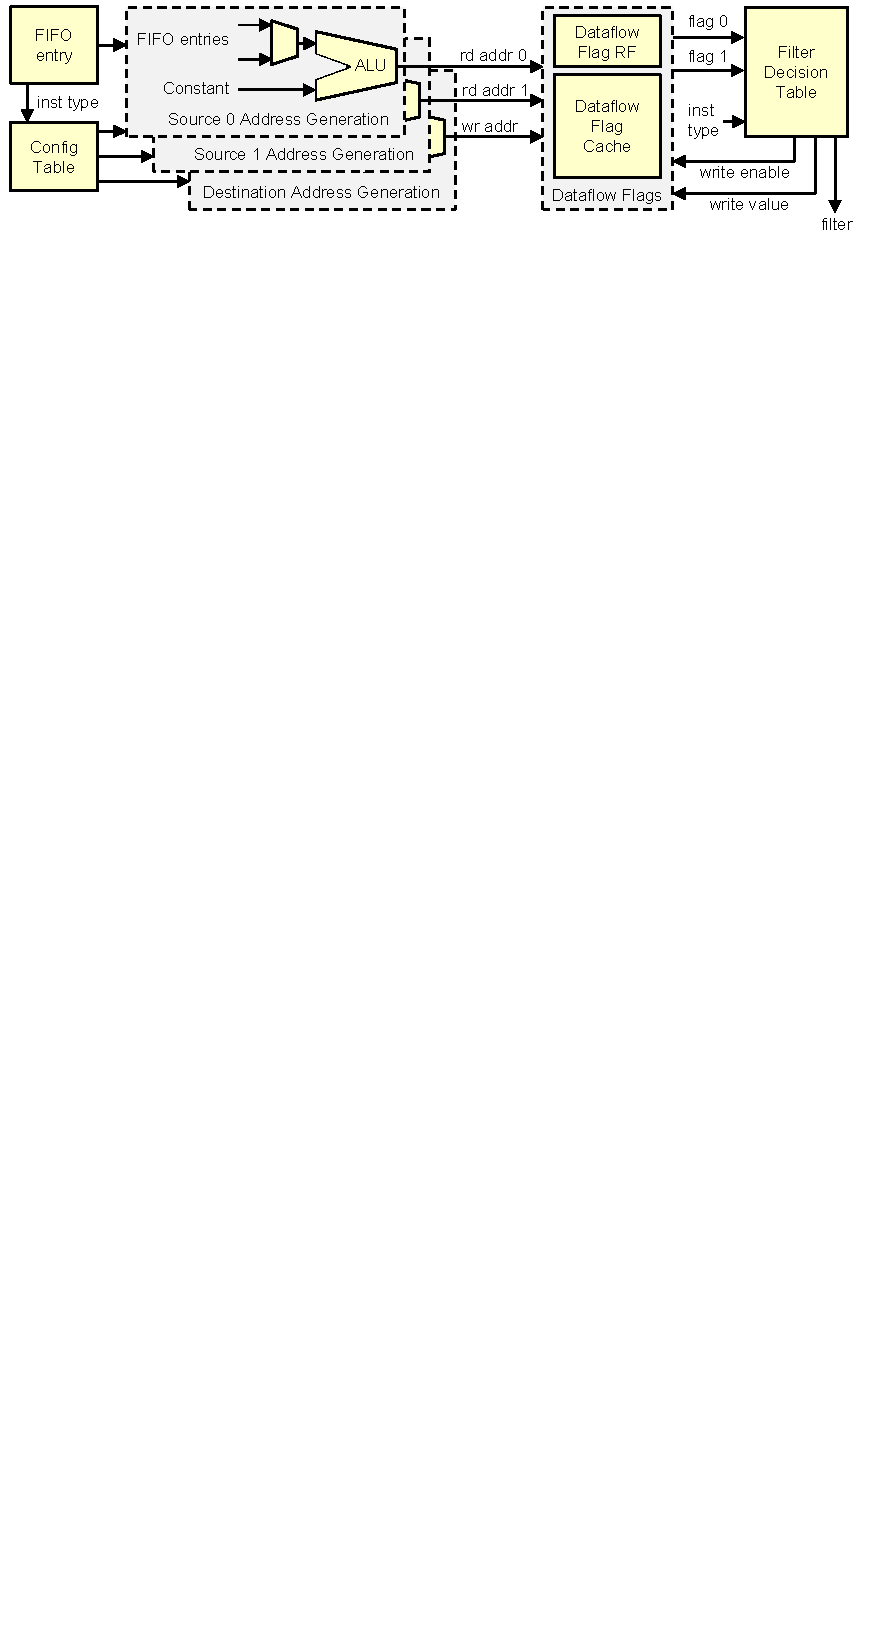
\includegraphics{monitoring_dift_drop/figs/dataflow_architecture.pdf}
    \caption{Hardware architecture of the dataflow engine.}
    \label{fig:monitoring_dift_drop.dropping.dataflow} 
  \end{center}
\end{figure}

Thus, the hardware acts effectively as a dataflow tracking engine in order to
track a 1-bit invalidation flag per metadata.
Figure~\ref{fig:monitoring_dift_drop.dropping.dataflow} shows a detailed block
diagram of this hardware module. The dataflow engine uses two address
generation units to read in up to two invalidation flags. These source
invalidation flags are used to decide whether a monitoring event should
filtered. A third address generation unit is used to optionally specify a
target to propagate the invalidation information. The module includes a
register file to store invalidation flags corresponding to register file
metadata. In addition, it uses a small memory-backed cache to handle
invalidation flags corresponding to memory metadata. The fact that the dataflow
flags are backed to memory differs from the design presented in
Chapter~\ref{chap:monitoring_hard_drop} for hard real-time systems. This allows
the architecture to have perfect invalidation information without aliasing. In
the worst-case, misses in the dataflow flag cache can cause high overheads for
dropping. However, we expect misses to be rare.

Since different monitoring operations are performed based on instruction type,
the dataflow engine is also configured based on instruction type. The source operands
and operation for the address generation units are set based on instruction
type. Note that the address generation units also take information from the
monitored event as inputs. Thus, in the same way that the monitoring core selects
metadata based on register indices or the memory address of the specific monitoring
event, the dataflow engine also reads the appropriate flags. In addition, the
filter decision table is configured based on instruction type to decide what
combination of input flags will lead to a filtered event and whether
propagation is required.

\subsection{Filtering Null Metadata}
\label{sec:monitoring_dift_drop.dropping.null_filtering}

% Null filtering code example
\begin{figure}
  \begin{center}
    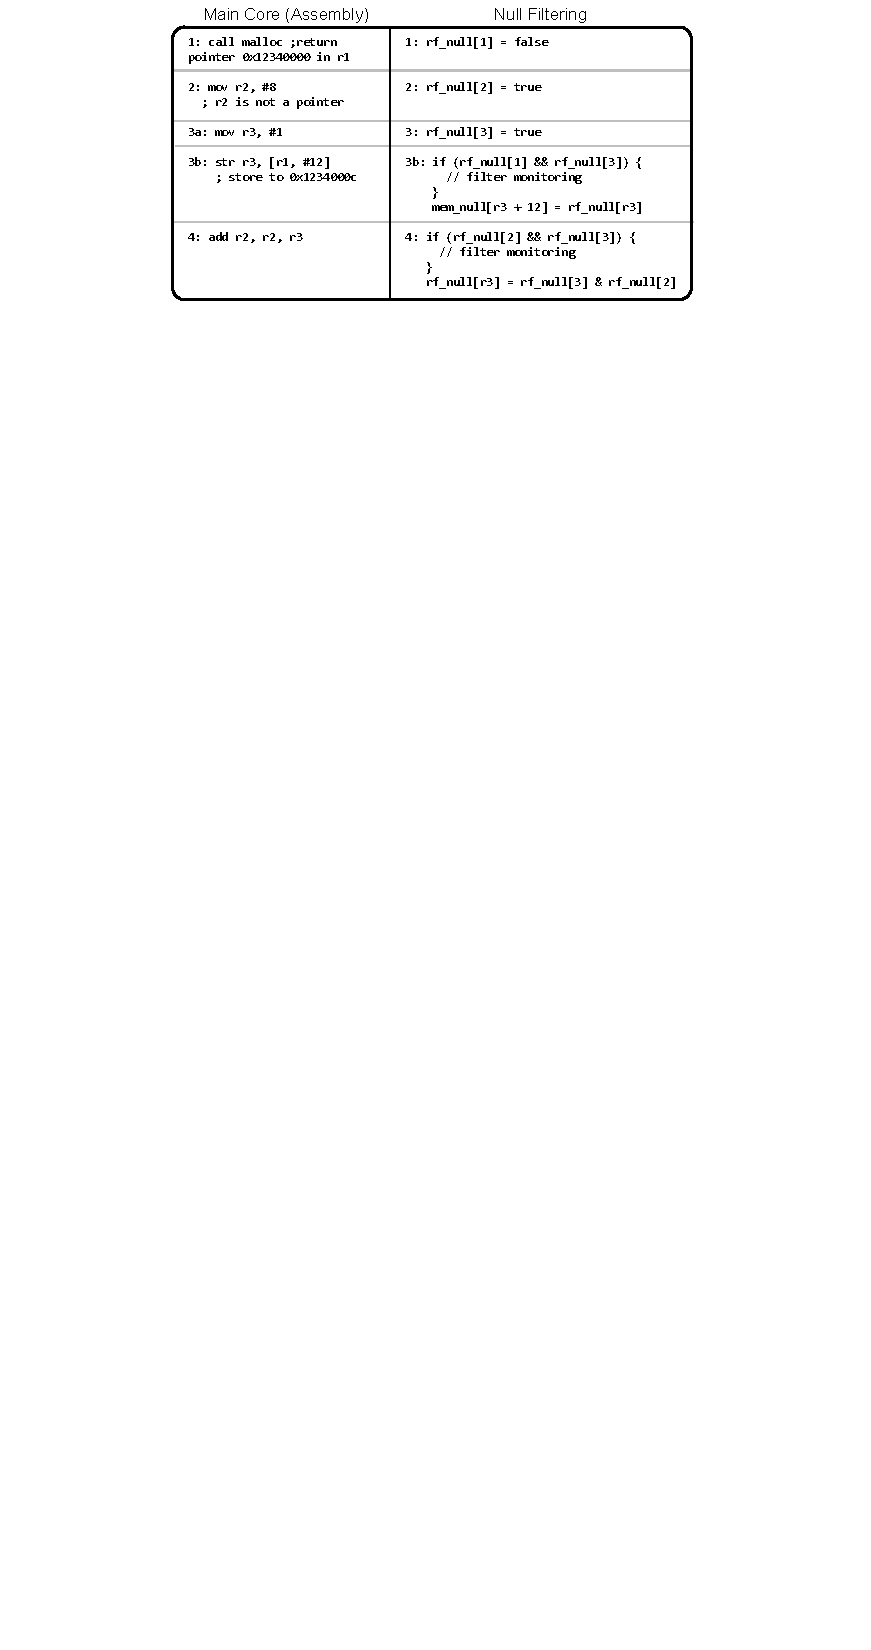
\includegraphics{monitoring_dift_drop/figs/example_null_filtering.pdf}
    \caption{Example of using information about null metadata to filter monitoring events.}
    \label{fig:monitoring_dift_drop.dropping.example_null} 
  \end{center}
\end{figure}

One way to reduce the number of monitoring events that must be handled by the
monitoring core is to filter out monitoring events that correspond to operating on null
metadata. Null metadata correspond to events that are not relevant to the
monitoring core. For example, Hardbound \cite{hardbound-asplos08} filters out
operations on non-pointer (i.e., no base and bounds metadata) instructions
since it is not relevant to array bounds checking. More recently, FADE
\cite{fade-hpca14} has been proposed as a general hardware module to perform
this null metadata filtering for a variety of monitoring schemes. Our
architecture is able to support this null metadata filtering with a small
modification.

Figure~\ref{fig:monitoring_dift_drop.dropping.example_null} shows an example of
how this null filtering operates.  Here, the main core's code has been slightly
modified from Figure~\ref{fig:monitoring_dift_drop.dropping.example_full} and
on line 2, {\tt r2} is no longer set as an array pointer.  Without null
metadata filtering, the instruction for line 4 would be forwarded to the
monitoring core since the system does not know whether {\tt r2} contains a pointer
address or not. However, if we use a 1-bit flag to mark {\tt r2} as null when
it is loaded with a constant, then we can propagate this null information and
filter out monitoring for line 4.

The operations performed by null filtering are almost identical to the
operations needed for invalidation shown in
Figure~\ref{fig:monitoring_dift_drop.dropping.example_invalid} except for a
small change in the propagation policy. Instead of taking a logical OR of the
source invalidation flags to determine whether monitoring can be skipped, null
metadata filtering takes a logical AND of the source null flags.  Thus, we can
easily enable this null metadata filtering on our architecture by extending the
dataflow flags to be two bits wide. One bit is used to keep track of
invalidation information while the second bit is used to keep track of null
information. All flags are initialized to null and the filter decision table is
extended with the propagation and filtering decision rules for null metadata
filtering.  The result is a single hardware design that enables both partial
monitoring and null metadata filtering.

